\begin{problem}{/images/problems/pic.jpg}{Right Triangles}Two right triangles $ABZ$ and $DBZ$ are given with the edges lengths below: 

\begin{itemize}
\item $\bar{ZA}=33$

\item $\bar{BD} =16$

\item $\bar{BZ}=65$
\end{itemize}
What is the the length of $\bar{TH}$.

\begin{center}
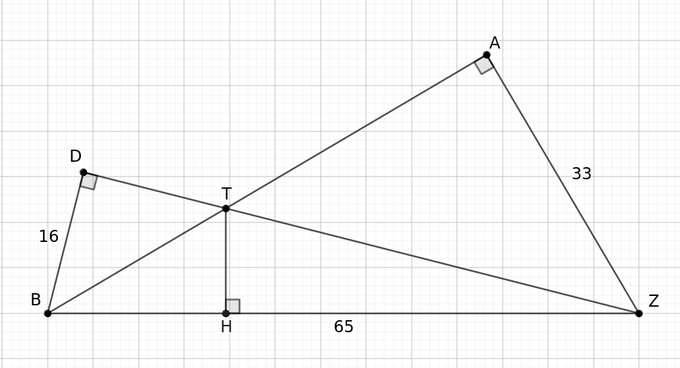
\includegraphics[width=9cm]{/images/problems/36_biruni.png}
\end{center}

Link to the problem on Twitter:  \url{https://twitter.com/Riazi_Cafe/status/1701844480939397217}\end{problem}
\begin{solution}
The answer is equal to $y \approx 11.53613$.\\[0.2cm]
According to the Pythagorean theorem, we have $\bar{AB}=56$ and $\bar{DZ}=63$. Considering $B$ as the origin, we formulate the lines $\bar{AB}$ and $\bar{DZ}$ as below. The $y$ coordinate of the intersection of these two lines is equal to the answer. %A function of a line can be written by having the slope and a point of that line. The slope of the line is equal to the tangent of its angle with the $x$ axis in the positive direction.

$$\begin{align}
\left.
\begin{aligned}
BA:& y = \frac{33}{56} x \\
DZ:& y = -\frac{16}{63}(x - 65)
\end{aligned}
\right\}
\quad &\implies \quad
x \approx 19.57647, y \approx 11.53613
\end{align}$$
\end{solution}
